\documentclass{standalone}
\usepackage{tikz}
\usepackage{mathptmx}
\usetikzlibrary{arrows,arrows.meta,calc,shapes,positioning,matrix}
\usepackage{tikzsymbols}

\begin{document}

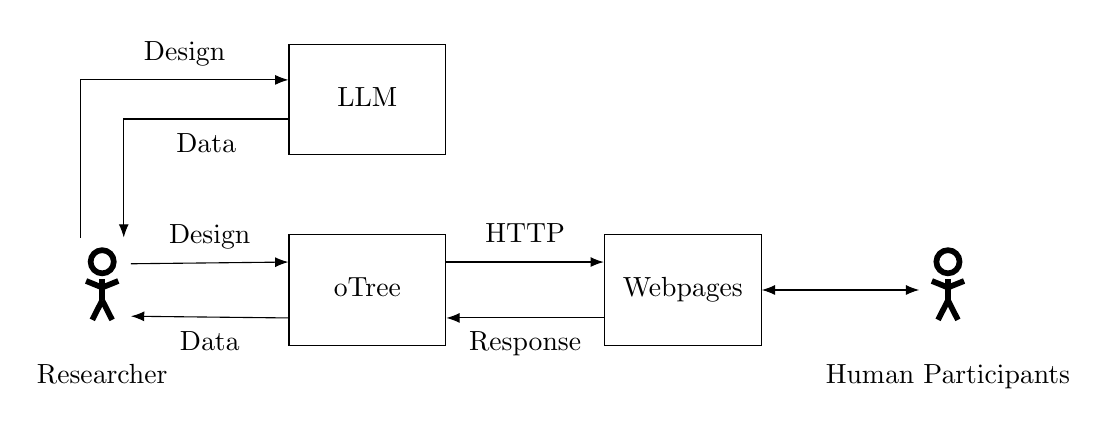
\begin{tikzpicture}[
    block/.style={rectangle, draw, text width=5em, text centered, minimum height=4em},
    line/.style={draw, -Latex},
    every node/.append style={
        execute at end node={\strut},
    }
]

% Blocks
\node[block] (otree) {oTree};
\node[block, above=	1cm of otree] (llm) {LLM};
\node[block, right=2cm of otree] (webpages) {Webpages};
\node[right=2cm of webpages] (participants) {\Strichmaxerl[4]}  {};
\node[left=2cm of otree] (researcher){\Strichmaxerl[4]} {};

% Lines
\draw[line] ($(researcher.east)!0.5!(researcher.north east)$) -- node[above] {Design} ($(otree.west)!0.5!(otree.north west)$);
\draw[line] ($(otree.west)!0.5!(otree.south west)$) -- node[below] {Data} ($(researcher.east)!0.5!(researcher.south east)$);
\draw[line] ($(otree.east)!0.5!(otree.north east)$) -- node[above] {HTTP} ($(webpages.west)!0.5!(webpages.north west)$);
\draw[line] ($(webpages.west)!0.5!(webpages.south west)$) -- node[below] {Response} ($(otree.east)!0.5!(otree.south east)$);
\draw[line, Latex-Latex] (participants) -- (webpages);
\draw[line] ($(researcher.north)!0.75!(researcher.north west)$) |- node[pos=0.75,above] {Design} ($(llm.west)!0.35!(llm.north west)$);
\draw[line] ($(llm.west)!0.35!(llm.south west)$) -| node[pos=0.25,below] {Data} ($(researcher.north)!0.75!(researcher.north east)$);

% Labels
\node[below=0.1cm of participants] {Human Participants};
\node[below=0.1cm of researcher] {Researcher};

\end{tikzpicture}
\end{document}